% !TEX root = ./CA_solution.tex

\section*{3장 - 연습문제 풀이}

\subsection*{연습문제 \ref{ex-3-1}}

$\gamma_1 = \cos t + i\sin t$, $\gamma_2 = \cos (2t) + i\sin (2t)$,
$\gamma_3 = \cos t - i\sin t$이므로
$k=1,2,3$ 각각의 경우 모두 $(\Re(\gamma_k(t)))^2 + (\Im(\gamma_k(t)))^2=1$이다.
$\gamma_k$의 상은 중심이 $0$이고 반지름이 $1$인 원 $\mathbb T$에 있다.
$\theta \in [0,2\pi)$에 대하여 $z = \exp(i\theta)$이면,
$z = \gamma_1(\theta) = \gamma_2(\theta/2) = \gamma_3(2\pi - \theta)$이다.
따라서 $\mathbb T$위의 모든 점은 $\gamma_1, \gamma_2, \gamma_3$ 각각에 의한 상에
속한다.
\begin{align*}
\int_{\gamma_1} \dfrac1z dz &= \int_0^{2\pi} \dfrac1{\exp(it)}\cdot i\exp(it)dt = 2\pi i, \\
\int_{\gamma_2} \dfrac1z dz &= \int_0^{2\pi} \dfrac1{\exp(2it)}\cdot 2i\exp(2it)dt = 4\pi i, \\
\int_{\gamma_3} \dfrac1z dz &= \int_0^{2\pi} \dfrac1{\exp(-it)}\cdot (-i)\exp(-it)dt = -2\pi i.
\end{align*}

\subsection*{연습문제 \ref{ex-3-2}}

실함수 $x,y$에 대하여 $\gamma(t) = x(t) +iy(t)$, $t\in[0,1]$라 하자.
또한, $u,v$를 각각 함수 $f$의 실수부와 허수부라 하면,
\begin{align*}
f'(\gamma(t))\cdot\gamma'(t)
&= \left( \dfrac{\partial u}{\partial x}(x(t),y(t)) +
i \dfrac{\partial v}{\partial x}(x(t),y(t)) \right) (x'(t) + iy'(t)) \\
&= \dfrac{\partial u}{\partial x}(x(t),y(t)) \cdot x'(t) - \dfrac{\partial v}{\partial x}y'(t) \\
&\qquad +i\left( \dfrac{\partial u}{\partial x}(x(t),y(t)) \cdot y'(t) + \dfrac{\partial v}{\partial x}x'(t) \right) \\
&= \dfrac{\partial u}{\partial x}(x(t),y(t)) \cdot x'(t) + \dfrac{\partial u}{\partial y}y'(t) \\
&\qquad +i\left( \dfrac{\partial v}{\partial y}(x(t),y(t)) \cdot y'(t) + \dfrac{\partial v}{\partial x}x'(t) \right) \\
&\qquad\qquad \text{(코시-리만 방정식을 적용함)} \\
&= \dfrac d{dt} u(x(t), y(t)) + i \dfrac d{dt} v(x(t),y(t)) \quad\text{(연쇄법칙을 적용함)} \\
&= \dfrac d{dt} (u(x(t), y(t)) + i v(x(t),y(t))) = \dfrac d{dt} f(\gamma(t)).
\end{align*}

\subsection*{연습문제 \ref{ex-3-3}}

원형경로 $\gamma$를 $\gamma(t) = 2\exp(it)$, $t\in[0,2\pi]$라 하자.
\begin{itemize}
\item[(1)] 
\begin{align*}
\int_\gamma (z+\bar z) dz & = \int_0^{2\pi} (2\exp(it) + 2\exp(-it))\cdot 2i \cdot \exp(it) dt \\
&= 4i\int_0^{2\pi} (\exp(2it) +1)dt - 4i\cdot 0 + 4i\cdot 2\pi = 8\pi i.
\end{align*}
\item[(2)] 
\begin{align*}
\int_\gamma (z^2-2z+3) dz & = \int_0^{2\pi} (4\exp(2it) - 4\exp(it)+3)\cdot 2i \cdot \exp(it) dt \\
&= \int_0^{2\pi} i(8\exp(3it) - 8\exp(2it) + 6\exp(it))dt  = 0+0+0 =0.
\end{align*}
\item[(3)] 
\begin{align*}
\int_\gamma xy dz & = \int_0^{2\pi}  2\cos t\cdot 2\sin t \cdot 2i \cdot(\cos t +i\sin t) dt \\
&= 4i\int_0^{2\pi} (\sin (2t))(\cos t + i\sin t)dt \\
&= 4i\int_{-\pi}^\pi \underbrace{(\sin(2t))\cos t}_{\text{기함수}} dt
- 2\int_0^{2\pi} (\cos t - \cos(3t))dt \\
&=0 - 2(0-0) = 0.
\end{align*}
\end{itemize}

\subsection*{연습문제 \ref{ex-3-4}}

\begin{itemize}
\item[(1)] $\gamma(t) =(1+i)t$, $t\in[0,1]$이므로,
$\dint_\gamma \Re(z)dz = \dint_0^1 t(1+i)dt = \dfrac{1+i}2$. 
\item[(2)] $\gamma(t) =1+\exp(it)$, $t\in[-\pi/2,0]$이므로, 
\begin{align*}
\int_\gamma \Re(z) dz &= \int_{-\pi/2}^0 (\cos t)i\exp(it)dt
= \int_{-\pi/2}^0 i(\cos t)^2 -(\cos t)(\sin t)dt \\
&= \int_{-\pi/2}^0 \left( i\dfrac{\cos(2t)+1}2 - \dfrac{\sin(2t)}2 \right) dt \\
&= 0 + i\cdot \dfrac12 \cdot \dfrac \pi2 + \dfrac12 = \dfrac12 + i\dfrac\pi4.
\end{align*}
\item[(3)] $\gamma(t) =t+it^ 2$, $t\in[0,1]$이므로,
\[
\int_\gamma \Re(z) dz  = \int_0^1 t\cdot(1+2it)dt = \dfrac12 + 2i\cdot\dfrac13 
=\dfrac12 + \dfrac23i.
\]
\end{itemize}

\subsection*{연습문제 \ref{ex-3-5}}

이항정리에 의하여
\[
(1+z)^n = \sum_{\ell = 0}^n  {n \choose \ell} z^\ell 1^{n-\ell} 
\sum_{\ell = 0}^n  {n \choose \ell} z^\ell.
\]
$0\le k \le n$에 대하여,
\[
\dfrac{(1+z)^n}{z^{k+1}} =\sum_{\ell = 0}^n  {n \choose \ell} z^{\ell-k-1}
\]
이므로
\begin{align*}
\dfrac1{2\pi i} \int_C \dfrac{(1+z)^n}{z^{k+1}}dz
&= \dfrac1{2\pi i} \int_C \sum_{\ell = 0}^n  {n \choose \ell} z^{\ell-k-1} dz \\
&  \sum_{\ell = 0}^n  {n \choose \ell} \dfrac1{2\pi i} \int_C  z^{\ell-k-1}dz
= {n \choose k}.
\end{align*}

\subsection*{연습문제 \ref{ex-3-6}}
\begin{itemize}
\item[(1)]
$U_f, V_f, U_g, V_g:[a,b] \to \mathbb R$에 대하여
$f(\gamma(t))\gamma'(t) = U_f(t) + iV_f(t)$,
$g(\gamma(t))\gamma'(t) = U_g(t) + iV_g(t)$, $t\in[a,b]$라고 하자.

\begin{align*}
\int_\gamma (f+g)(z)dz
&= \int_a^b (f+g)(\gamma(t))\cdot \gamma'(t)dt \\
&= \int_a^b \left( f(\gamma(t))\cdot \gamma'(t) + g(\gamma(t))\cdot \gamma'(t) \right) dt\\
&= \int_a^b (U_f(t) + U_g(t)) dt + i \int_a^b (V_f(t) + V_g(t)) dt \\
&= \int_a^b U_f(t)dt + \int_a^b V_f(t)dt + i\int_a^b V_f(t)dt + i\int_a^b V_g(t)dt \\
&= \int_\gamma f(z)dz + \int_\gamma g(z)dz.
\end{align*}

\item[(2)] $\alpha = p+iq$ ($p,q\in\mathbb R$)이고
$U,V:  [a,b] \to \mathbb R$에 대하여
$f(\gamma(t))\gamma'(t)  = U(t) + iV(t)$, $t\in[a,b]$라 하자.
그러면,
\begin{align*}
\int_\gamma (\alpha\cdot f)(z) dz
&= \int_a^b (p+iq)(U(t) + iV(t))dt \\
&= \int_a^b(pU(t) - qV(t))dt + i\int_a^b (pV(t) + qU(t))dt \\
&= p \left(\int_a^b U(t)dt + i \int_a^b V(t)dt \right)
+ iq\left(\int_a^b U(t)dt + i \int_a^b V(t)dt \right) \\
&= (p+iq)\left(\int_a^b U(t)dt + i \int_a^b V(t)dt \right)
= \alpha \cdot \int_\gamma f(z)dz.
\end{align*}
\end{itemize}

\subsection*{연습문제 \ref{ex-3-7}}

$-(-\gamma): [a,b] \to \mathbb C$는 다음 식으로 주어진다.
\[
(-(-\gamma))(t)= (-\gamma)(a+b-t) = \gamma(a+b-(a+b-t)) = \gamma(t),
\quad t\in[a,b].
\]
따라서 $-(-\gamma) = \gamma$이며, 그림으로 보면 직관적으로 명백하다.

\subsection*{연습문제 \ref{ex-3-8}}

$\gamma(b) = (-\gamma)(a)$이므로
$\gamma$와 $-\gamma$는 결합가능한 경로이다.
\[
\int_{\gamma+(-\gamma)} f(z) dz = \int_\gamma f(z) dz + \int_{-\gamma} f(z)dz
=  \int_\gamma f(z) dz - \int_\gamma f(z) dz = 0.
\]

\subsection*{연습문제 \ref{ex-3-9}}

$\gamma:[0,1] \to \mathbb C$를 $\gamma(t) = (1+i)t$, $t\in [0,1]$이라 하자.
피타고라스 정리를 쓰면, $\gamma$의 길이는 $\sqrt{1^2+1^2} = \sqrt{2}$.

\begin{figure*}[h!]
\begin{center}
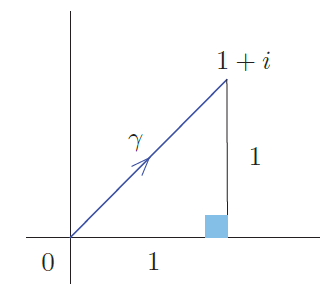
\includegraphics[width=0.3\textwidth]{./figs/fig-s-0-8}
\end{center}
%\caption{$\left\{ z \in\mathbb C \,:\, z\ne0, \dfrac\pi4 < |\Arg(z)| < \dfrac\pi3 \right\}$}
%\label{fig-5-14}
\end{figure*}

또한 $|(\gamma(t))^2| = |t+it|^2 = 2t^2$이고,
$\max\limits_{t\in[0,1]} |(\gamma(t))^2| = 2\cdot 1^2 = 2$.
따라서
\[
\left| \int_\gamma z^2dz \right|
\le \left( \max\limits_{t\in[0,1]} |(\gamma(t))^2|  \right) \cdot
(\text{$\gamma$의 길이})
= 2\sqrt{2}.
\]
직접 계산하면,
\begin{align*}
\int_\gamma z^2 dz = \int_0^1 (t+it)^2\cdot(1+i)dt
= \int_0^1 (1+i)^3t^2dt = \dfrac{(1+i)^3}3
\end{align*}
이므로
$\left| \dint_\gamma z^2 dz \right| = \dfrac{(\sqrt{3})^3}3 = \dfrac{2\sqrt{2}}3$.

\subsection*{연습문제 \ref{ex-3-10}}

\begin{align*}
{2n \choose n} = \left|  {2n \choose n} \right|
&= \left| \dfrac1{2\pi i}\int_C \dfrac{(1+z)^{2n}}{z^{n+1}}dz \right| \\
&\le \dfrac1{2\pi} \left( \max_{|z|=1} \left| \dfrac{(1+z)^{2n}}{z^{n+1}}\right| \right)
\cdot 2\pi\cdot 1 = \max_{|z|=1} \dfrac{|1+z|^{2n}}1 \\
&\le (1+1)^{2n} = 2^{2n} = 4^n.
\end{align*}

\subsection*{연습문제 \ref{ex-3-11}}

$F=U+iV$를 $\bar z \in \mathbb C$의 부정적분이라고 하자.
그러면,
\[
\dfrac{\partial U}{\partial x}  + i \dfrac{\partial V}{\partial x}
= \dfrac{\partial V}{\partial y} - i\dfrac{\partial U}{\partial y}
= F' = \bar z = x-iy.
\]

$x_0\in\mathbb R$을 고정하자. 그러면 $(x,y)\in\mathbb R^2$에 대하여
\[
V(x,y ) - V(x_0, y) = \int_{x_0}^x \dfrac{\partial V}{\partial x}(\xi, y )d\xi
= \int_{x_0}^x -y d\xi = -xy +x_0y.
\]
따라서 $V(x,y) = -xy + \varphi(y)$, $\varphi(y):+V(x_0,y_0) + x_0y$이면,
\[
x  = \dfrac{\partial V}{\partial y} = -x + \varphi'(y).
\]
즉, 모든 $x\in\mathbb R$에 대하여 $\varphi'(y) = 2x$인데
이는 분명 모순이다.
특히, $2\cdot 1 = 2 = \varphi'(y) = 2\cdot  0 = 0$.

\subsection*{연습문제 \ref{ex-3-12}}

$(fg)' = fg' + f'g$이므로
함수 $\zeta \mapsto f(\zeta)g'(\zeta) + f'(\zeta)g(\zeta)$는 
부정적분을 갖는다.
따라서 경로적분의 기본정리에 의하여
\[
\int_\gamma \left( f(\zeta)g'(\zeta) + f'(\zeta)g(\zeta) \right) d\zeta
= f(z)g(z) - f(w)g(w)
\]
이고 이를 정리하면 원하는 결과를 얻는다.

\subsection*{연습문제 \ref{ex-3-13}}

$\mathbb C$에서 $\sin' z = \cos z$이므로 $\cos z$는 부정적분을 갖는다.
따라서 경로적분의 기본정리에 의하여
\begin{align*}
\int_\gamma \cos z \, dz 
&= \sin i - \sin (-i) = 2\sin i = 2\dfrac{\exp(i\cdot i) - \exp(-i\cdot i)}{2i}
= \dfrac{e^{-1} - e^{1}}i \\
&= \left( e - \dfrac1e \right)i.
\end{align*}


\subsection*{연습문제 \ref{ex-3-14}}

$\mathbb C$에서  $\exp' z = \exp z$이므로
$0$과 $a+ib$를 잇는 경로 $\gamma$를 따라 적분하면
\[
\int_\gamma \exp z\, dz = \exp(a+ib) - \exp 0 = e^a(\cos b + i \sin b) -1
= e^a\cos b -1 +ie^a\sin b.
\]
 경로를 $\gamma(x) = (a+ib)x$, $x\in[0,1]$로 잡으면,
\[
\int_\gamma \exp z\, dz = \int_0^1 \exp(a+ib)\cdot (a+ib)dx
= \int_0^1 e^{ax}(\cos(bx) + i\sin(bx))(a+ib)dx.
\]
 따라서,
$(a-ib)\dint_\gamma \exp z\, dz = \dint_0^1 e^{ax}(\cos(bx) + i\sin(bx))(a^2+b^2)dx$이고,
\begin{align*}
(a^2+b^2) \int_0^1 e^{ax} \cos (bx)dx
&= \Re\left( (a-ib)\int_\gamma \exp z\, dz \right) \\
&= \Re((a-ib)(e^a\cos b -1 + ie^a\sin b)) \\
&= a(e^a\cos b -1) + be^a \sin b.
\end{align*}
즉,
$\dint_0^1 e^{ax}\cos(bx)\, dx = \dfrac{a(e^a\cos b - 1) + be^a\sin b}{a^2+b^2}$.

\subsection*{연습문제 \ref{ex-3-15}}

중심이 $0$이고 반지름 $r>0$인 원을 반시계방향으로 도는 닫힌경로 $C$를 생각하자.






%


